\documentclass[11pt,a4paper]{article}

\usepackage[utf8]{inputenc} 
\usepackage[T1]{fontenc} 
\usepackage{lmodern}
\usepackage[margin=2cm]{geometry}
\usepackage[german]{babel}
\usepackage{amsmath} 
\usepackage{graphicx} 
\usepackage{booktabs}
\usepackage{hyperref}
\hypersetup{
    colorlinks,
    citecolor=red,
    filecolor=black,
    linkcolor=black!20!blue!90!,
    urlcolor=black} 
\usepackage{nicefrac}
\usepackage[table]{xcolor}
\usepackage{tocloft}
\usepackage{array}

\newcolumntype{L}[1]{>{\centering\let\newline\\\arraybackslash\hspace{0pt}}m{#1}}

\setlength{\parindent}{0pt}
\setlength{\parskip}{1ex plus 0.5ex minus 0.5ex}

\definecolor{incolor}{rgb}{0.0, 0.0, 0.5}

\hbadness=99999

\newcommand{\refpy}[1]{Siehe Anhang: \textit{Rechnungen in Python} (\texttt{{\color{incolor}In [{\color{incolor}#1}]}})}
\newcommand{\dif}{\mathop{}\!\mathrm{d}}
\newcommand{\vphi}{\varphi}
\newcommand{\halftime}[4]{\begin{figure}[h]
\begin{minipage}{.#1\textwidth}#3\end{minipage}\begin{minipage}{.#2\textwidth}
\centering
#4\end{minipage}
\end{figure}}


\begin{document}


{
\centering 
\large 
Physiklabor für Anf\"anger*innen \\
Ferienpraktikum im Sommersemester 2018 \\[4mm]
\textbf{\LARGE 
Versuch 22: Kreiselpr\"azession
} \\[3mm]
(durchgef\"uhrt am 21.09.2018 bei Adrian Hauber) \\
Andréz Gockel, Patrick M\"unnich\\
\today \\[10mm]
}

\vspace{50pt}
\tableofcontents
\vspace{22pt}
\listoftables
\vspace{22pt}
\listoffigures
\pagebreak

\section{Ziel des Versuchs}

Dieser Versuch dient dazu, freie Rotation eines Systems mit von au\ss en wirkender Drehmomente darzustellen. Insbesondere wird hier auf Pr\"azession eingegangen. Dazu Nutzt man einen Kreisel, an dem Pr\"azession und Rotation betrachtet werden.

\section{Versuch}

\subsection{Theorie}

Starre K\"orper haben Tr\"agheitsmomente in Form eines Tensors. Bestimmte Achsen sind jedoch vielsagend. Diese formen einen Tr\"agheitsellipsoid mit den Hauptachsen $I_A$, $I_B$ und $I_C$. Bei symmetrischen Kreisel, wie hier vorhanden, sind $I_B$ und $I_C$ gleich. $I_A$ ist das Tr\"agheitsmoment bez\"uglich der Figurenachse. Bei Kreiseln ist dieses gleichzeitig unsere gr\"o\ss te Komponente beim Tr\"agheitsellipsoid.

Tr\"agheitsmomente sind allgemein mit der Drehgeschwindigkeit $\vec{\omega}$ und dem Drehimpuls $\vec{L}$ verbunden:

\begin{equation}
\vec{L}=I\vec{\omega}
\end{equation}

Sto\ss t man einen an der Figurenachse gebundenen Kreisel an, so wirkt ein Drehmoment:

\begin{equation}
\vec{M}=\vec{r}\times\vec{G}=\frac{\dif\vec{L}}{\dif t}\label{m=rg}
\end{equation}

$\vec{r}$ bezeichnet hier den Vektor vom Unterst\"utzungspunkt zum Schwerpunkt ud $\vec{G}$ die Gewichtskraft im Schwerpunkt.

Da dies sich nur in der senkrechten Komponente \"andert, \"andert sich der Betrag des Drehimpulses nicht. Die einzige \"Anderung ist die Richtung, welche zu einer Drehbewegung in der Senkrechte f\"uhrt. Diese Bewegung wird als Pr\"azession bezeichnet, mit der Winkelgeschwindigkeit $\vec{\omega}_P$. Zusammen mit der Drehgeschwindigkeit $\vec{\omega}_F$ um die Figurenachse ergibt sich die momentane Drehgeschwindigkeit $\vec{\omega}$.

Bei einem pr\"azedierenden Kreisel gibt es also eine Kreisbewegung mit Radius $L\sin\phi$ mit $\phi$ als Winkel zwischen $\vec{L}$ und der vertikalen Achse. Die Rotationsgeschwindigkeit hat einen Betrag von $\omega_P=\nicefrac{\dif\vphi}{\dif t}$, wobei $\vphi$ der azimutale Winkel ist. Die \"Aenderung des Drehimpulses ist also eine Richtungs\"anderung $\dif\vphi=\frac{\dif L}{L\sin\phi}$. Mit diesem Wissen kommen wir also zu

\[
\omega_P=\frac{\dif\phi}{\dif t}=\frac{\dif L}{\dif tL\sin\phi}
\]

Dies k\"onnen wir umschreiben zu

\begin{equation}
\frac{\dif\vec{L}}{\dif t}=\vec{\omega}_P\times\vec{L}.
\end{equation}

Mit (\ref{m=rg}) kommen wir zu der Gleichung

\begin{equation}
\vec{r}\times\vec{G}=\vec{\omega}_P\times\vec{L}\label{rgisoml}
\end{equation}

Da wir in diesem Versuch mit einem schnell rotierenden Kreisel arbeiten, also $\omega_F>>\omega_P$ gilt n\"aherungsweise $\sin(\vec{r},\vec{G})=\sin(\vec{\omega}_P,\vec{L})$. Als n\"achstes schreiben wir (\ref{rgisoml}) f\"ur die Betr\"age der Vektoren um:

\begin{equation}
rG\sin(\vec{r},\vec{G})=\omega_PL\sin(\vec{\omega}_P,\vec{L}).
\end{equation}

Nutzen wir unsere N\"aherung aus, so k\"onnen wir schreiben

\begin{equation}
rG\approx\omega_AL\approx\omega_FL.
\end{equation}

Hier ist $\omega_A$ die Drehgeschwindigkeitskomponente, die mit $\omega_B$ entlang zweier Haupttr\"agheitsachsen des Kreisels verl\"auft und sich mit $I_A$ und $I_B$ zusammen zu $\vec{L}$ vektoriell addieren lassen. 

Mit $L\approx I\omega_A\approx I\omega_F$ k\"onnen wir sagen, dass $L\approx\omega_P\omega_AI\approx I\omega_P\omega_F$. Damit kommen wir auf unsere gesuchte Gleichung

\begin{equation}
I_A=\frac{rG}{\omega_F\omega_P},\label{eqIA}
\end{equation} 

welche wir f\"ur unsere Rechnungen ben\"otigen.

\subsection{Aufbau}


\halftime{5}{5}{Es wurde ein Kreiselrad mit verstellbarer Kreiselachse verwendet. Dieser wurde auf ein Stativ mit einer drehbaren Halterung die es ermöglichte eine Präzessionsbewegung zu durchlaufen. Eine Federwaage wurde verwendet um die Masse des Kreisels zu bestimmen. Es wurden zwei Stoppuhren benutzt um jeweils die Präzessionsfrequenz und die Rotationsfrequenz zu messen. 
}{\fbox{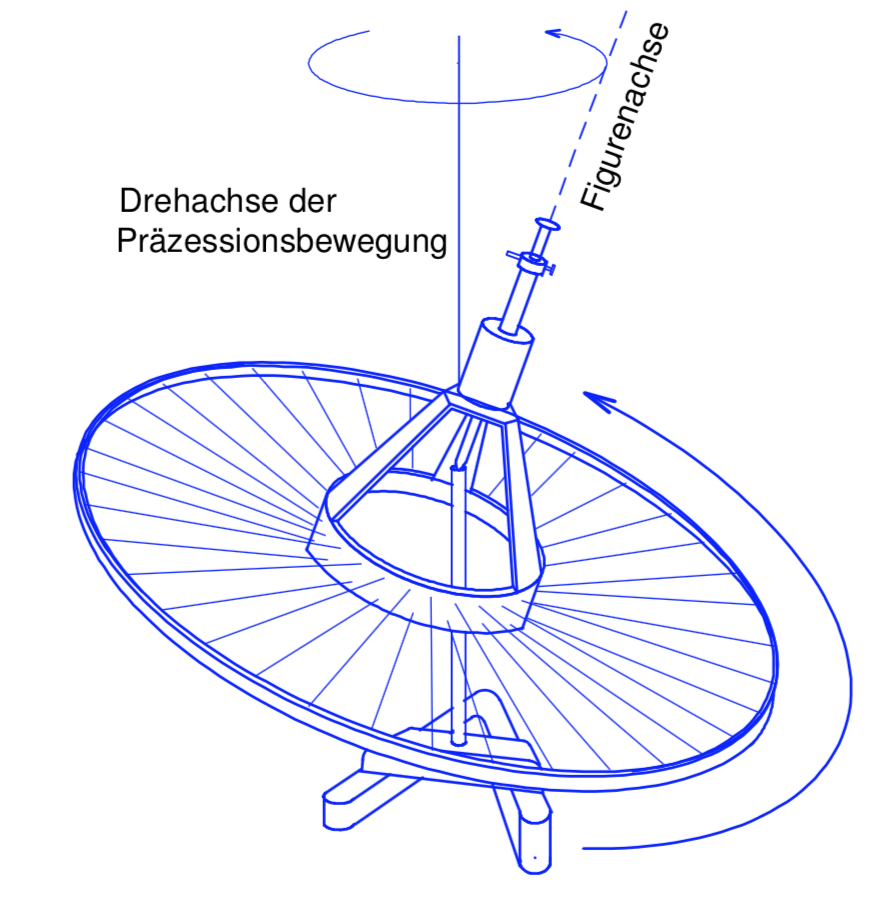
\includegraphics[width=0.9\textwidth]{Krpr}}
   \renewcommand\thefigure{B1}
\caption[Präzessierender Kreisel]{Präzessierender Kreisel \cite{Anleitung}}
\label{Pic:1}}

\subsection{Durchführung}

Zuerst wurde Masse des Kreisels gemessen. Zunächst wurde die Kreiselachse eingestellt, dann wurde das Kreiselrad angehoben und per hand im Uhrzeigersinn gedreht. Der rotierende Kreisel wurde dann vorsichtig auf die Halterung platziert und gekippt. Dann wurden 10 Rotationen zeitlich gemessen, und eine Präzessionsbewegung. Dies wurde für 10 verschiedene Kreiselachsen vier mal durchgeführt. Die Drehrichtung der Präzessionsbewegung wurde jedesmal notiert. Es konnten nur die Drehrichtung bestimmt werden für die Einstellungen wo der Schwerpunkt zu nahe dem Unterstützungspunkt war.

\subsection{Auswertung}

Erstmals ist es wichtig zu wissen, dass unser gesuchtes $I_A$ eine Konstante ist. Wollen wir diese mit (\ref{eqIA}) finden, so brauchen wir $r$, $m$, $g$, $\omega_F$ und $\omega_P$. Die Masse $m$ k\"onnen wir leicht messen und wir bekommmen als Ergebnis $(4.52\pm0.020$)\,kg. F\"ur $g$ verwenden wir einfach $9.81\,\nicefrac{\mathrm{m}}{\mathrm{s}^2}$. $\omega_F$ und $\omega_P$ k\"onnen wir \"uber die Periodendauer T berechnen: 
\[
\omega=\frac{2\pi}{T}.
\]

Uns fehlt also nur noch $r$. Da $I_A$ eine Konstante ist, k\"onnen wir aus der Gleichung (\ref{eqIA}) schlie\ss en:
\begin{equation}
r=\frac{\omega_F\omega_P}{G}\label{eqgraph}
\end{equation}
F\"ur die rechte Seite der Gleichung ist alles gemessen. Wir k\"onnen dies in eine Graphik auftragen, in der wir dann einen linearen Zusammenhang sehen werden. Wir folgern, dass $r$ wohl aus unserem eingestellten Abstand $x$ summiert mit einem Offset $x_0$ besteht.

Nutzen wir f\"ur als lineare Gleichung f\"ur eine Ausgleichsgrade von dne Messpunkten
\[
y=a+bx,
\]
so k\"onnen wir unser $x_0$ als $-\frac{a}{b}$ festlegen.

Um unser $a$ und $b$ zu finden, sowie auch die Standardunsicherheiten von $y$, $a$ und $b$, nehmen wir folgende Formeln zunutze:

\begin{equation}
a=\frac{\sum x_i^2\sum y_i-\sum x_i\sum x_iy_i}{n\sum x_i^2-(\sum x_i)^2}
\end{equation}
\begin{equation}
b=\frac{n\sum x_iy_i-\sum x_i\sum y_i}{n\sum x_i^2-(\sum x_i)^2}
\end{equation}
\begin{equation}
s=\sqrt{\frac{1}{n-2}\sum^n_{i=1}[y_i-(a+bx_i)]^2}
\end{equation}
\begin{equation}
\Delta a=s\sqrt{\frac{\sum x_i^2}{n\sum x_i^2-(\sum x_i)^2}}
\end{equation}
\begin{equation}
\Delta b=s\sqrt{\frac{n}{n\sum x_i^2-(\sum x_i)^2}}
\end{equation}
Unsere letzte Messreihe hat eine zu gro\ss e Abweichung, was zu einer ungenaueren Geraden f\"uhrt. Erl\"auterung des Grundes dessen ist in der Diskussion zu finden. Die resultierende Graphik ist im Anhang. Wir nutzen also die letzte Messreihe nicht aus.
Um dann unseren Offset $x_0$ und seine Standardunsicherheit zu finden, rechnen wir also
\[
x_0=\frac{-a}{b}
\]
\[
\Delta x_o=x_0\times\sqrt{\left(\frac{\Delta a}{a}\right)^2+\left(\frac{\Delta b}{b}\right)^2}
\]
Aus unseren Messwerten, welche in Tabelle (\ref{Tab:X}) im Anhang gefunden werden kann, folgern wir also:
\begin{itemize}
\item Offset $x_0=4.70$
\item Unsicherheit Offset $\Delta x_0=0.20$
\item $\nicefrac{\Delta x_0}{x_0}=0.04=4\%$
\end{itemize}

Um das gesuchte $I_A$ zu berechnen, nutzen wir Gleichung (\ref{eqIA}). Damit bekommen wir als Mittelwert
\[
I_A=(14.5\pm0.6)\,\mathrm{kgcm}^2
\]

Den Fehler des Mittelwerts berechnen wir \"uber die allgemeine Formel:

\begin{equation}
s_x=\sqrt{\frac{1}{n-1}\sum_{i=1}^n(x_i-\overline{x})^2}.\label{uncertainty1}
\end{equation}

\section{Diskussion}

%Y U NO LAST MEASUREMENT

Da $I_A$ eine Konstante ist, k\"onnen wir aus der Gleichung f\"ur $I_A$ schlussfolgern, dass
\[\frac{\omega_F\omega_P}{G}\]
linear verlaufen muss. Tragen wir dies mit allen Messwerten auf, so bekommen wir den Graph, der im Anhang als Abbildung (\ref{Abb:2}) gefunden werden kann.

Dies sieht zwar relativ linear aus, jedoch k\"onnen wir ohne dem letzten Punkt einen klar lineareren Verlauf feststellen. Dies l\"asst sich dadurch erkl\"aren, dass die letzte Messreihe bei $x=10$ durchgef\"uhrt wurde und unser Offset $x_0=4.70$ ist. Da 10 im Vergleich zu den anderen Messwerten schon weit entfernt ist von 4.70, ist klar, dass dessen Werte nicht besonders gut sein wird.

Unser Ergebnis (zur Wiederholung: $I_A=(14.5\pm0.6)\,\mathrm{kgcm}^2$) verf\"ugt \"uber keinen Literaturwert, mit dem wir das vergleichen k\"onnen. Da unser Fehler bei 4\% liegt deutet dies darauf, dass er genau sein sollte.

Es ist jedoch ein systematischer Fehler vorhanden, unzwar, dass die Reibung des Kreisels die Drehgeschwindigkeit verlangsamt. Wie stark dessen Einfluss ist kann man rausfinden, indem man die Periodendauer \"uber einen Zeitraum mehrmals misst. 
Bei einem Zeitraum von 10\,s wurde bei dem hier verwendeten Kreisel gemessen, dass sich die Periodendauer von 10 Umdrehungen von 6.3\,s bzw. 5.6\,s auf 7.1\,s bzw. 6.1\,s gesinkt ist. Dies entspricht jeweils 13\% bzw. 9\%. Es ist also durchaus m\"oglich, dass die Reibung den Wert beeinflusst. Betrachten wir die Gleichung zum Berechnen von $I_A$,
\[
I_A=\frac{rG}{\omega_F\omega_P},
\]
so k\"onnen wir klar sehen, dass $I_A$ von zwei von $T$ abh\"angigen Werten, $r$, $\omega_F$ und $\omega_P$ abh\"angt. Setzen wir $T$ zu dem 1.10-Fachen, so erhalten wir mit der gleichen Rechnung wie zuvor $(17.5\pm0.7)$\,kgcm$^{2}$.

Dieser Wert ist das $(1.20\pm0.05)$-Fache von unserem vorher berechneten Wert.

Vergleichen wir diese Werte mit der folgenden Formel:
\begin{equation}
t=\frac{\vert x_0-y_0\vert}{\sqrt{u_x^2+u_y^2}},\label{abw}
\end{equation}
so erhalten wir $t=4.13$. Dies ist au\ss erhalb des erw\"unschten $t<2$ Bereichs. Diese beiden Werte sind also unvertr\"aglich. Zwar ist keines der beide ein Literaturwert, jedoch k\"onnen wir dadurch deutlich erkennen, dass der durch die Reibung entstehende Fehler einen gro\ss en Einfluss hat.



%Dies wurde in diesem Fall gemessen, und es wurde festgestellt, dass diese Reibung \"ueber einen Zeitraum von 10\,s die Drehung um circa 10\% verlangsamt. Dies k\"onnte also einen Einfluss haben.







\pagebreak

\section{Anhang: Tabellen und Diagramme}

\begin{figure}[h]
\centering
\fbox{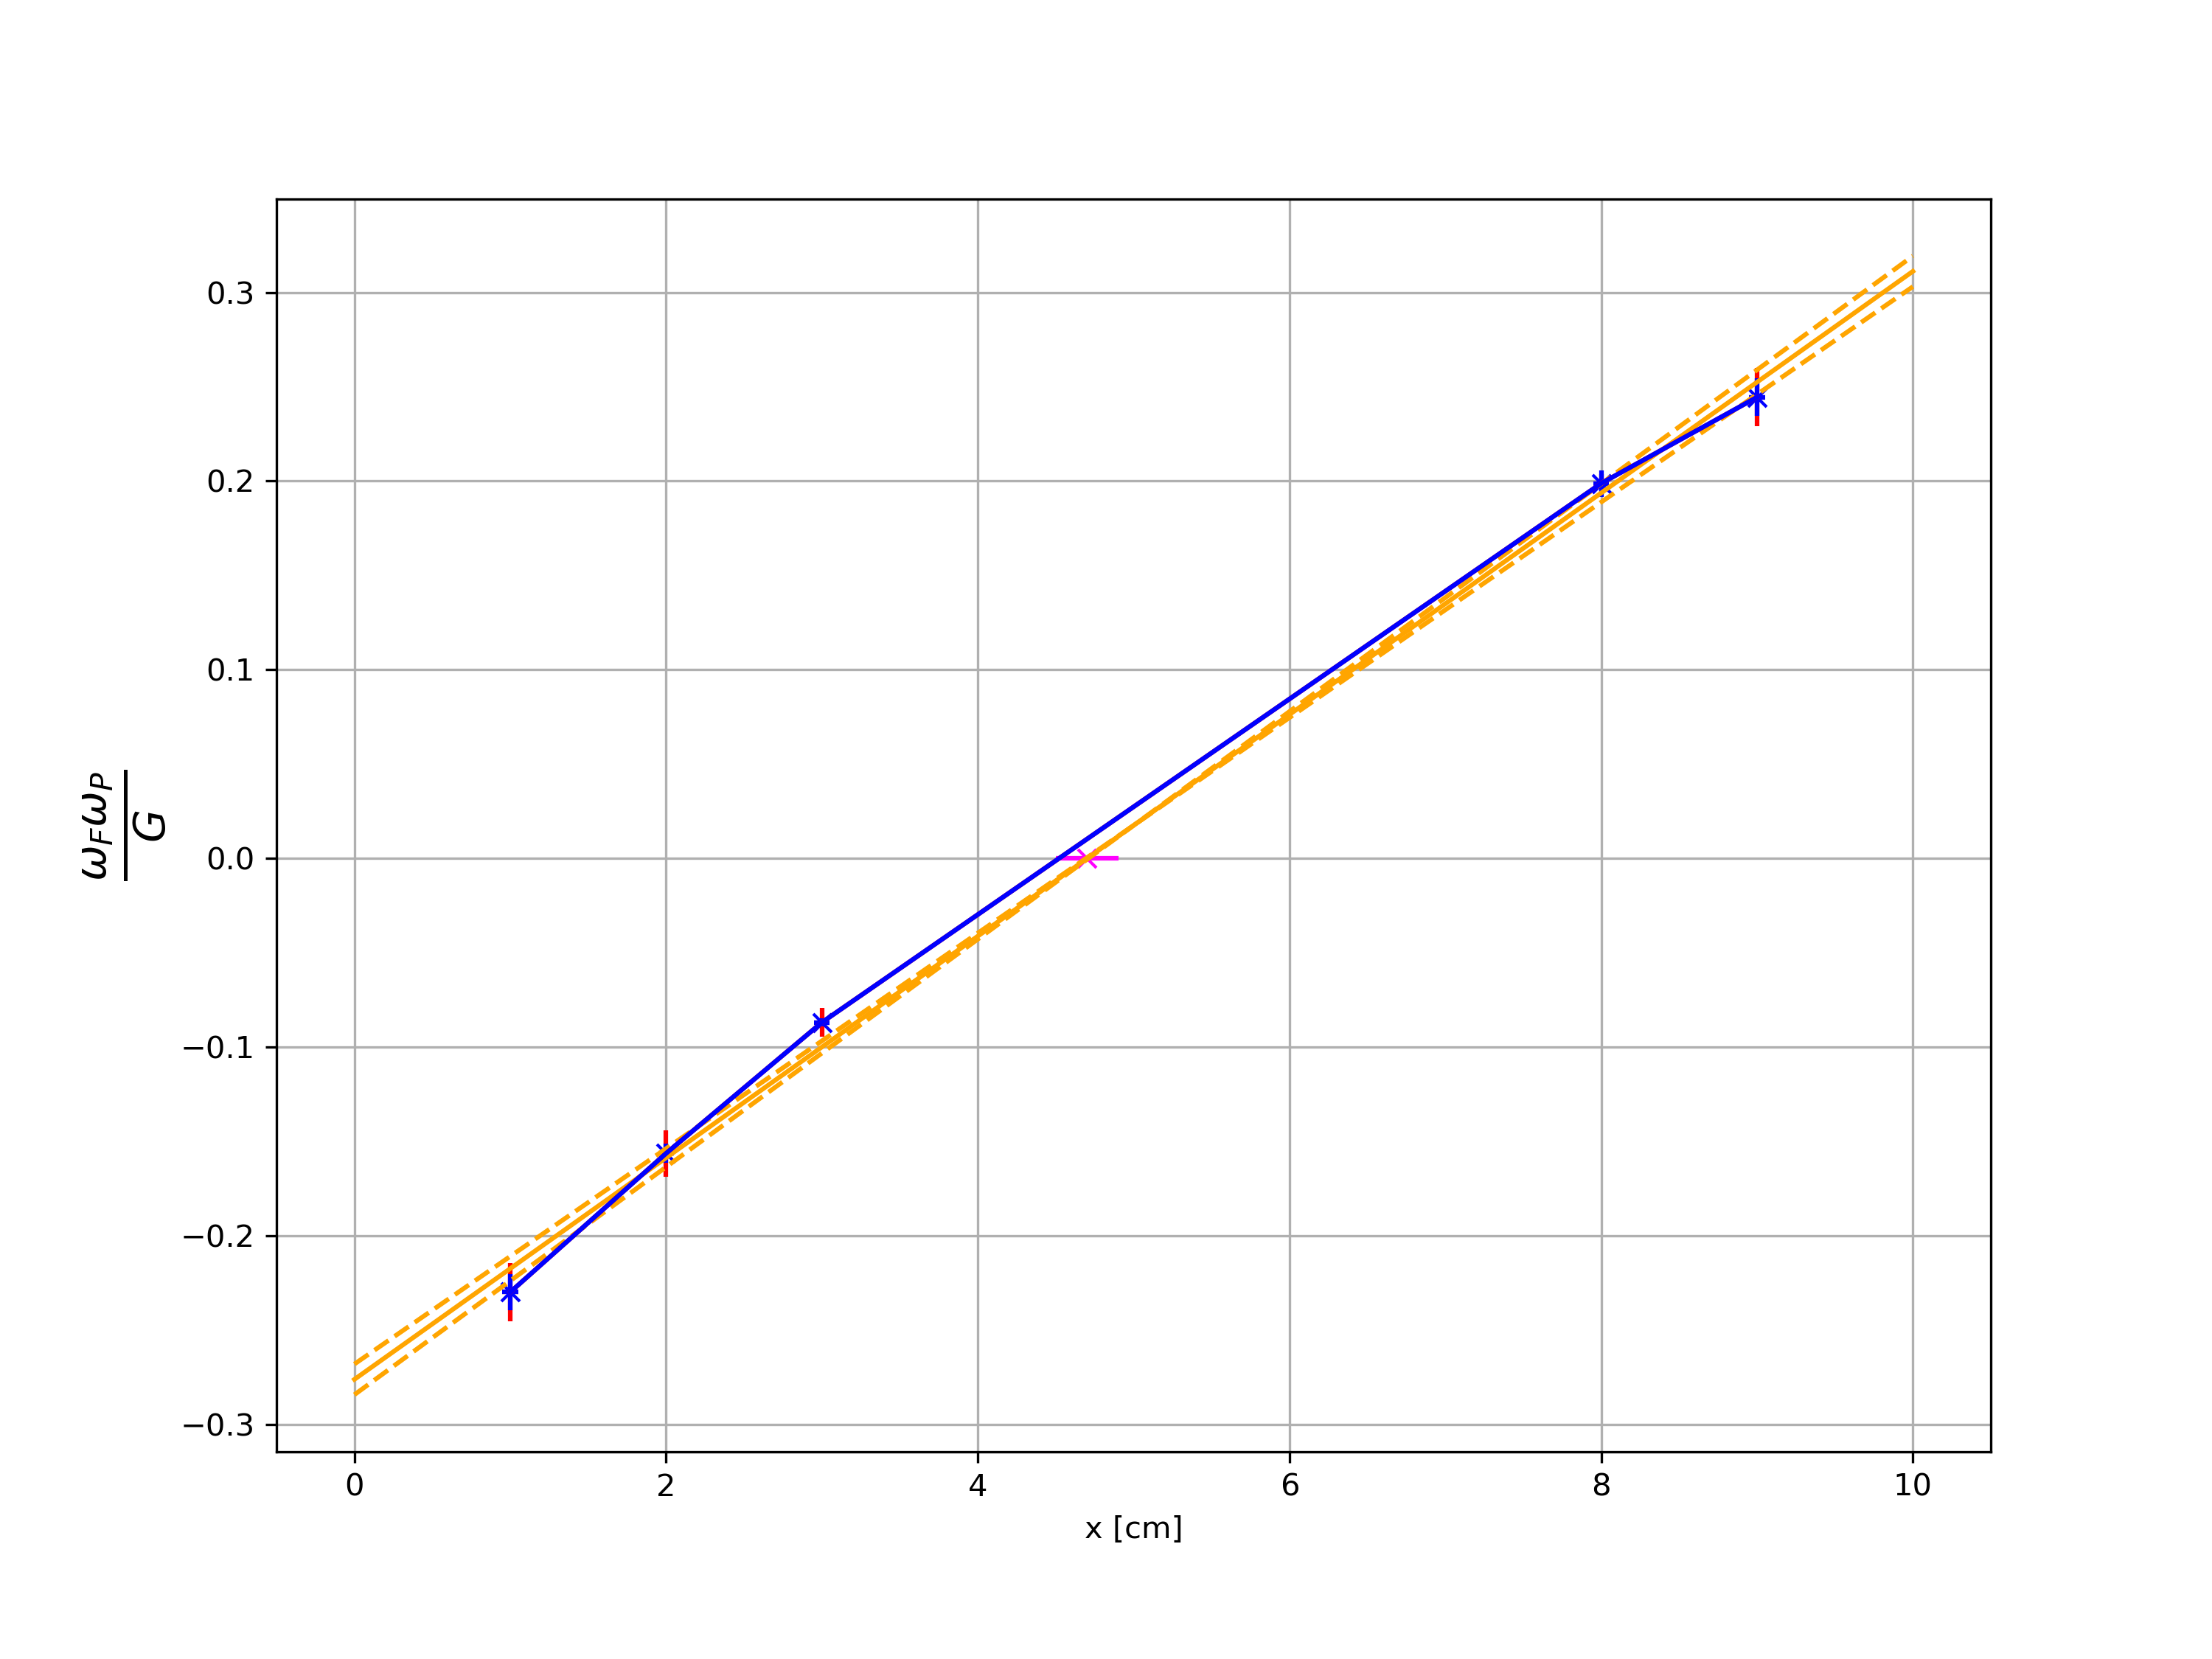
\includegraphics[width=0.8\textwidth]{discluding_10.png}}
\renewcommand\thefigure{1}
\caption[Graphik Messpunkte mit Ausgleichsgerade]{Ausgleichsgerade}
\label{Abb:1}
\end{figure}

\begin{figure}[h]
\centering
\fbox{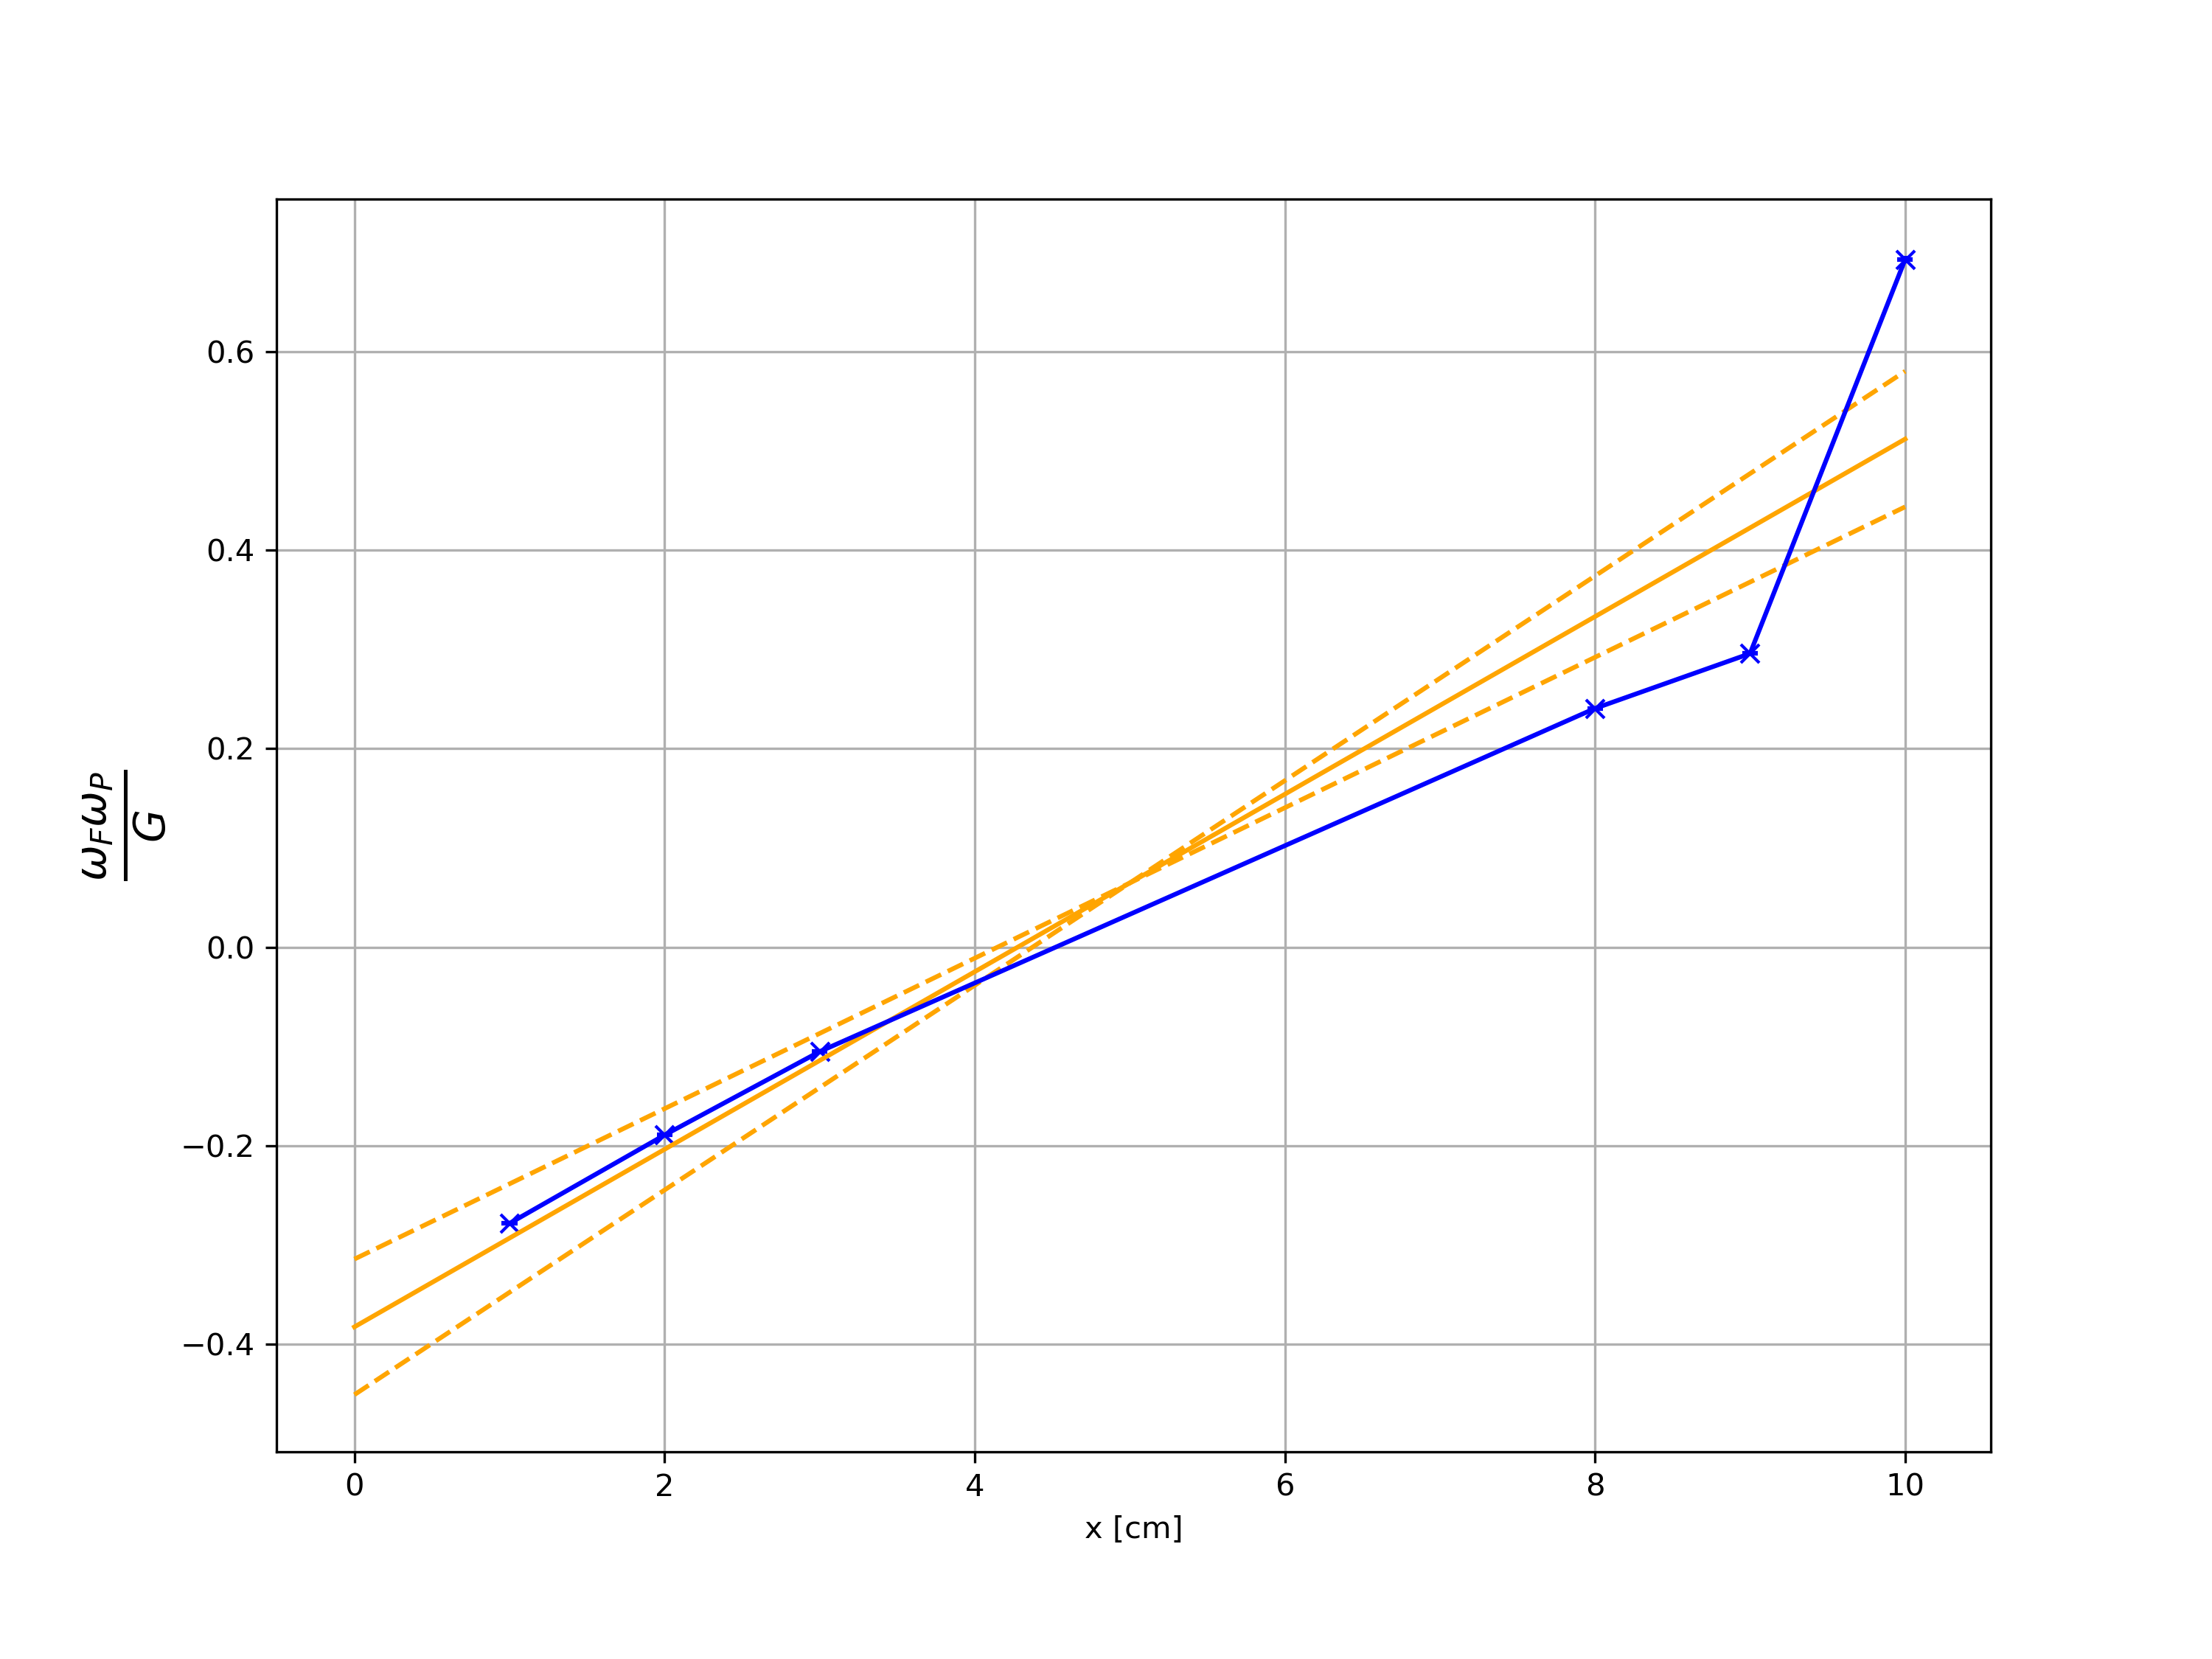
\includegraphics[width=0.8\textwidth]{including_10.png}}
\renewcommand\thefigure{2}
\caption[Vergleichsgraphik]{Vergleichsgraphik}
\label{Abb:2}
\end{figure}

\begin{table}[h]
\centering
\caption{Messwerte} \vspace{11pt}
$\begin{array}{l}
\textrm{Unsicherheiten:}\\
\textrm{Zeit: } \pm 0.3 \textrm{s}\\
\textrm{Länge: } \pm 0.05 \textrm{cm}\\
\end{array}$
\begin{tabular}{ r L{3cm} L{3cm} }
\toprule
$l$\textrm{ in cm} & \textrm{Präzession umlaufdauer\textrm{ in s}} & \textrm{10 Rotationen umlaufdauer}\textrm{ in s} \\
\midrule
1 & 6.6 & 5.1\\
1 & 4.7 & 6.9\\
1 & 3.6 & 8.1\\
1 & 7.9 & 4.2\\
\hline
2 & 6.5 & 6.7\\
2 & 6.7 & 6.7\\
2 & 7.0 & 6.0\\
2 & 9.4 & 5.5\\
\hline
3 & 13.7 & 6.8\\
3 & 14.4 & 6.2\\
3 & \phantom{0}9.8 & 7.8\\
3 & 13.4 & 6.1\\
\hline
8 & 5.7 & 6.4\\
8 & 6.6 & 5.5\\
8 & 5.6 & 6.6\\
8 & 6.4 & 6.0\\
\hline
9 & 5.1 & 5.7\\
9 & 4.7 & 6.5\\
9 & 4.1 & 8.0\\
9 & 6.3 & 4.5\\
\hline
10 & 1.7 & 6.7\\
10 & 2.7 & 5.0\\
10 & 3.9 & 3.6\\
10 & 3.2 & 4.0\\
\bottomrule
\end{tabular}
\phantom{$\begin{array}{l}
\textrm{Unsicherheiten:}\\
\textrm{XXXX: } \pm XX \textrm{XX}\\
\end{array}$}
\label{Tab:X}
\end{table}

%\begin{figure}[p]
%\centering
%\fbox{\includegraphics[width=0.8\textwidth]{NAME}}
%\renewcommand\thefigure{BX}
%\caption[XXXX]{XXXX}
%\label{Abb:X}
%\end{figure}

\begin{thebibliography}{9}
\bibitem{Uncertainties}''Correlations between variables are automatically handled, which sets this module apart from many existing error propagation codes.'' - https://pythonhosted.org/uncertainties/
\bibitem{Anleitung} Physikalisches Institut der Albert-Ludwigs-Universität Freiburg (Hrsg.) (08/2018): Versuchsanleitungen zum Physiklabor für Anfänger*innen, Teil 1, Ferienpraktikum im Sommersemester 2018.
\end{thebibliography}

\end{document}